\documentclass[tikz,border=5]{standalone}
\usepackage[utf8]{inputenc}
\usepackage{xcolor}
\usepackage{tikz}
\usetikzlibrary{patterns,positioning,arrows,arrows.meta,calc,shapes,pgfplots.groupplots,fit,backgrounds}

\begin{document}

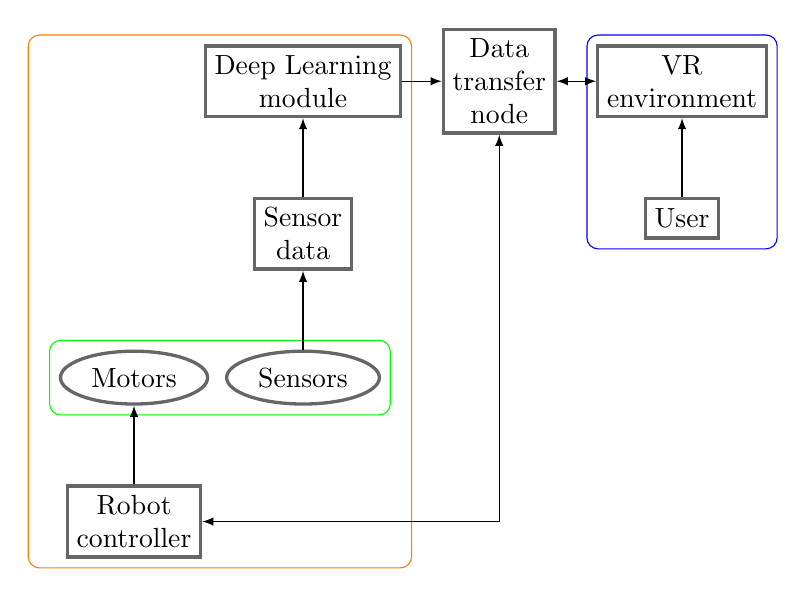
\begin{tikzpicture}[squarednode/.style={rectangle, draw=black!60,  very thick, minimum size=5mm},every text node part/.style={align=center},   dot/.style={
        % fill=blue,
        circle,
        minimum size=3pt}, ellipsenode/.style={ellipse, draw=black!60,  very thick, minimum size=5mm}]
    %Nodes
    \node[squarednode]      (realworld)                              {Sensor \\ data};
    \node[ellipsenode]        (sensors)       [below=of realworld] {Sensors};

    \node[ellipsenode]        (motors)       [left= 0.2cm of sensors] {Motors};
    \node[squarednode]        (DNN)       [above=of realworld] {Deep Learning \\ module};
    \node[squarednode]        (tcp)       [right= 0.5cm of DNN] {Data\\transfer\\node};
    \node[squarednode]        (vr)       [right = 0.5cm of tcp] {VR  \\ environment};
    \node[squarednode]        (user)       [below=of vr] {User};
    \node[dot] (e) at (-3.2,1.5) {};
    \node[dot] (f) at (0.8,-3) {};

    % boxes
    \node[squarednode]        (motion)       [below=of motors] {Robot \\ controller};
    \node (box) [draw=orange,rounded corners,fit = (realworld) (DNN)  (motion) (e) (f)] {};
    \node (box) [draw=blue,rounded corners,fit = (user) (vr)] {};
    \node (box) [draw=green,rounded corners,fit = (sensors) (motors)] {};
    
    %Lines
    \draw[-latex] (sensors.north) -- (realworld.south);
    \draw[-latex] (realworld.north) -- (DNN.south);
    \draw[-latex] (DNN.east) -- (tcp.west);
    \draw[latex-latex] (tcp.east) -- (vr.west);
    \draw[-latex] (user.north) -- (vr.south);
    \draw[latex-latex] (tcp.south) |- (motion.east);
    \draw[-latex] (motion.north) -| (motors.south);


    \end{tikzpicture}

\end{document}